\documentclass[]{report}   % list options between brackets
\usepackage[textwidth=15cm, textheight=20cm]{geometry}              % list packages between braces
\usepackage{graphicx}
\usepackage{float}
\usepackage{cite}
\usepackage{url}
\renewcommand\thesection{\arabic{section}}

\begin{document}

\title{QR Codes for Security and Authentication}
\author{Andy Hansen\\\\
Supervised by David Eyers}
\date{Sep 19, 2014}
\maketitle
\tableofcontents

\section{Introduction}
QR codes have been around since 1997, but have been used for little more than putting website URLs into a physically scannable form. The aim of my project is to see if there are interesting ways we can use QR codes as a way of authenticating a user and setting up a secure channel of communication between a user and the services they wish to access. We plan to use Android smartphones as a means of generating and displaying the user's credentials in QR code form, so that they may be scanned by the service and grant them access without the user having to enter their username and password directly where it could be compromised. The user's details will sometimes be combined with context information proving that the intended user is the one scanning the QR code or codes.

In this report I am going to look at similar systems that have been created, give an overview of my experimental infrastructure, explain what my system is currently capable of, and give the advantages of technologies I have picked.

\section{Background}    
\subsection{Kerberos}
%todo: look at that paper I found that talks about kerb really good, talk about ticket renewal
%todo show a diagram on how Kerberos authentication works
%Kerberos \cite{Kerb} is a computer network authentication protocol which allow nodes to prove their identity to one another in a secure way. It uses ‘tickets’ as its mechanism to prove identity, a valid user will have a ticket to give to the service they wish to access. Kerberos allows both the user and the server to identify each other. When a user logs into the Kerberos key distribution center (KDC) they are given a ticket granting ticket (TGT). The TGT is presented by the user when they wish to access a restricted service, if the service accepts the user's TGT they will be given a ticket specific to the service when they can then use to access it securely. Kerberos is single sign-on meaning that once a user gets their TGT, they will not need to login again until it expires.
Kerberos \cite{Kerb} is a computer network authentication protocol which allow nodes to prove their identity to one another in a secure way. Any entities within the Kerberos system are known as principals. A principal refers to either a user accessing the network from a workstation, or a network service running on a host. Principals are contained in network groups called realms. Each realm is controlled by two servers which are the ticket granting server (TGS) and the authentication server (AS). Usually these two servers will be contained on the same host which is known as the key distribution center (KDC).

When a user wants to access a service principal on the network they will need a ticket for that principal which shows they are allowed access it. The negotiation of tickets is done using the ticket granting ticket (TGT) the user gets by authenticating themselves to the AS. This will happen in a few steps, and if successful will result in the user getting a TGT from the TGS. The TGT is used to negotiate additional tickets without the user needing to re-enter their password. To begin with the user sends the AS a plaintext message containing their user ID, the TGS ID, their IP address, and the lifetime they want to have for the ticket. The IP address can be left null if the user wants to allow the ticket to be used from any machine. The AS will check the user is in the database, and if they are will randomly generate a TGS session key which is used for encryption between the user's machine and the TGS. It then sends back two messages to the user:
\begin{itemize}
\item Message A: Encrypted with the user's secret key and contains: the TGS ID, the timestamp, the lifetime, and the TGS session key.
%The purpose of this message is that allows the user to get the TGS session key by decrypting it with their password.
\item Message B: Is the TGT, it is encrypted using the TGS secret key, and contains: the user ID, the TGS ID, the timestamp (which will match the message A's lifetime), the network address if one was given, the lifetime of the TGT, and the TGS session key.
\end{itemize}

The user now has two messages from the AS, the TGT which they cannot decrypt, and the message A that they can decrypt. Message A tells them about the contents of the TGT and gives them the TGS session key. The user is then prompted to enter their password so that message A can be decrypted, and once entered the user's secret key is determined by adding the user's principal e.g.\ user@REALM-NAME.COM, to the end of the password and hashing it. If the password was entered correctly then the user's machine will be able to decrypt message A. The TGT is stored encrypted in the users credintials cache. If message A was decrypted successfull the user can now use the TGS session key, and the TGT to request tickets for service principals. The user's password does not leave their workstation in this exchange, which is one of the reasons why Kerberos is so secure.

When the user needs a ticket for a particular service prinicipal it will send two messages to the TGS:
\begin{itemize}
\item Message C: This is plaintext and contains the ID of the requested service principal, and the TGT from message B.
\item Message D: The user's ID and a timestamp, this message is encrypted with the TGS session key and is known as the Authenticator.
\end{itemize}

The TGS will check the database to see if the requested service principal exists. If is does, the users TGT is decrypted using the TGS's secret key, then the Authenticator is decrypted using the session key contained in the TGT. Now that the TGS has the decrypted messages it will do a series of things: check the user ID from the Authenticator matches the TGT, make sure the timestamp of the Authenticator is within two minutes of the TGT, make sure the TGT is not expired, check to see that the Authenticator is not in the cache (this would indicate a replay attack), and check the IP address matches the source's IP address. If any of these checks fail then the user is sent the corrosponding error message. If successful then the TGS will generate a service session key, and send the user two messages:

\begin{itemize}
\item Message E: The service ticket for the principal. It contains the user ID, the service name, the users network address if it was given in message B, a timestamp, the valid time for the ticket, and the service session key. This message is encrypte using the service's secret key.
\item Message F: This message contains the principal service name, a timestamp, the validity time, and the principal services's session key. It is encrypted using the TGS session key.
\end{itemize}

The user's workstation decrypts message F using the TGS session key it obtained earlier, it now has access to the principal service's session key. Similarly to the TGT, the service ticket cannot be decrypted by the user because it was encrypted using that service's secret key.



\subsection{QR Codes}
%TODO talk about error correction and how it isn't really needed in my project since the QR codes aren't printed so there is no chance of part of the code being destroyed
A QR, or Quick Response code \cite{QR} is a specially formatted image which is designed to be quickly read by a camera. QR codes come in a range of versions, a version refers to how many rows and columns there are in the code, a high version code is going to be able to store more information, but will also be harder to read. QR codes store data using one of four different modes: numeric only, alphanumeric, byte/binary (ISO8859-1), and kanji. The mode affects how many characters can be stored within the QR code e.g. A numeric only code will be able to store more than the alphanumeric code.

\begin{figure}[H]
\centering
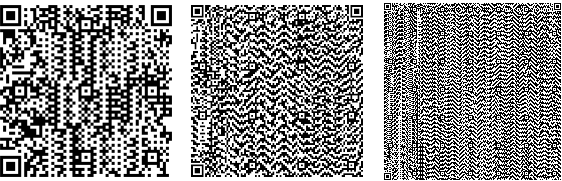
\includegraphics[width=9cm]{QRCodes.png}
\caption{QR code versions 10, 20, and 40 respectively.}
\end{figure}

\section{Research}
\subsection{Smart Cards}
%SmartCards http://isrc.ccs.asia.edu.tw/www/myjournal/P013.pdf
%remote authentication usually uses smart cards or a mobile phone with QR codes
% \cite{SmartCards} \cite{SmartNoPassword}
%TODO tamper resistent stuff
Passwords are a common means of authentication, though sometimes they not enough. For a long time smart cards were seen as a good way of supplimenting the password. (ref)  Smart cards provide the user with a physical resource they can present the computer in conjunction with their password to prove that they are correct user. In lower security settings it can also be appropriate to authenticate a user for just scanning their card. Smart cards are good because they are often a closed technology, it is difficult for a user to alter them. The disadvantage is that a lot is involved in getting a user a smart card. The card needs to be created and have the user's information put onto it.

%TODO: reword, or find the term for non-passive
Smart cards will also come in two varieties, passive or active. A passive card will only be able to store information, and cannot do computations. Once created it will not be able to change what it contains. Active cards have a small amount of processing power and storage which allows them to do more complex operations. Papers have been written for both kinds of cards for authentication.

\subsection{QR Codes on Mobile Phones}
In recent years there has been more research into QR codes for authentication. The increased popularity of smartphones is a likely cause of this because a smartphone provides a platform for a user to retrieve, store, and display the QR codes. Users will often have their smartphone on them, so it is a safe assumption that the location of the users smartphone is the same as their location.

Though QR code/smartphone schemes do not offer a clear cut improvement over smart cards they do have some advantages. There is a reduced cost to all parties, the user does not need an extra device for authentication, they just need to have their smartphone with them. This is both a good and a bad thing, the admin of the system does not need to issue each user a smart card, but smartphones are a lot easier to tamper with than a smart card. When using a smartphone based scheme the admin will need to be more cautious with checks to make sure a user is who they claim to be. Smartphones have a wide range of sensors available such as GPS, Wi-Fi, screen, keyboard, and Bluetooth. Authentication applications can take advantage of this and do checks such as making sure a user is in the location they claim to be when authentication is taking place. A smart card implementation would require additional hardware to track a user's position, and a user is less likely to carry a GPS device with them than a smartphone.

\section{My Progress}
\subsection{Infrastructure}
%todo change to a footnote
My current infrastructure involves three servers that are all running Ubuntu 14.04. The first server is used as the Kerberos key distribution center (KDC) running version 5 and a domain name server that uses Bind version 9 \cite{Bind}. The second server hosts an Apache web server which can be only be accessed with a valid Kerberos ticket from the KDC server. At the moment the Apache server is playing the role of any possible future Kerberos enabled service. It is a good service to use when testing because there is instant visual feedback when it is working. The third is an SSH server and is used in a similar way to the Apache server, but to test command line applications. A use case that results in me being able to access the Apache or SSH server could be replaced with any other service such as access to my account from the user login GUI, or access to a secured file system.

%TODO change apache to someting else
I am using Kerberos because it is runs on all popular operating systems and has built in support in a lot of existing services such as Apache, SSH, and Samba. This means that when a service is configured to connect with the user's KDC, they can use their TGT to access restricted web pages, SSH into protected machines, and access specific folders. I am using Kerberos version 5 because it is the most recent and has resolved some security concerns that were present in version 4 \cite{KerbUpdate}. Kerberos is also useful because all tickets have an expiry time. This is important in my system because if a malicious user intercepts the QR codes then they can only abuse the tickets in the short time window before they expire. Kerberos is single sign-on which is useful in our QR code based system because the user can use the TGT to gain access to any new service they need without reentering their username and password. It is a protocol that is supported on all major operating systems and is well tested. Designing an authentication protocol myself it would require me to do all of the integration and testing which would take a long time without providing very much benefit.

In my project QR codes are going to be used as a primary communication channel between the user and their services. QR codes are a good option because they are easy to use, and hard to perform a man in the middle attack on. The malicious user would have to get a copy of all the user's QR codes before they could use them themselves. Getting a copy of the user's QR codes is especially difficult because a wise user would only ever have their QR codes on screen when they need to use them. Even if a user does end up accidently giving away a QR code, their attack will need the complete set of QR codes before they can actually use them in an attack.

%TODO change to the right thing
Unfortunately QR codes do not have support direct binary encoding. This means that Kerberos tickets (which are stored in binary) need to be converted to an alphanumeric format before being encoded. This means that before a ticket is encoded into a QR code it is first converted into base64. 

\subsection{Dynamic Grouping of Users}
Dynamic grouping of users is a concept which is used in two of my use cases. The idea is that a Kerberos enabled network has a set of groups who each have access to particular resources. A user needs to be a member of the group controlling the resources before they are given access. These groups can be set up to last indefinitely, or for short periods of time. The reason you may want to have a short term group is if you want resources protected for a majority of the time, but then open them up to users in a controlled way e.g.\ allowing users to use the meeting room printer for the duration of a meeting.

%TODO Which service?
Users are added to the group when they meet certain conditions e.g.\ they are near the resources, or they are part of a collaboration. Kerberos lacks native group control, so needs to be implemented by the service. My proposed system puts group support into Kerberos, so that there is a single control point for the groups, rather than each of the resources having to manage their own groups individually.

The point of the dynamic groups is that it gives the KDC a point of reference to see which users are currently meeting a certain condition, and thus are allowed to use particular resources. The condition could be anything, but in my use cases they reflect the user's location. By having this conditional access protecting resources it gives more control than traditional Kerberos would offer, it makes it harder for malicious users to abuse controlled resources because they need their, or the person who's account they have hijacked need to be meeting the condition before they can cause any harm.

%TODO clarify what is meant by scanning of QR codes.
There are many ways of saying where a user is, each fit for different situations. The three main ways considered are: locating the user with Wi-Fi, GPS, and scanning of QR codes which will come in two forms; user QR codes scanned by an admin, or QR codes scanned by the user.

\begin{itemize}

%TODO citation for WIFI triangluation
\item Wi-Fi: It is possible to triangulate a user’s position using multiple Wi-Fi routers. As long as the user is connected to the system's Wi-Fi then their position can be worked out within X meters, which means that the system would be able to detect which room a user is in. The problem with this system is that it requires Kerberos to be integrated with the routers. It also means there needs to be a database of MAC addresses so that when a device is in range, the right user is associated with it. This means that a MAC address could be spoofed but the malicious user would have to spoof the MAC address, be in the right location, and have the victim user's QR code tickets. This would be good for situations where a user needs to be confirmed to be in a room that does not need any kind of supervision.

%TODO GPS section needs all kinds of improvements
\item GPS: GPS would would similar to Wi-Fi. The signal would have to be coming from a smartphone, and there would need to be a way of telling who was sending which GPS signal and it can happen automatically. It is not accurate indoors, so cannot be used to identify if a user is in a particular room. Another problem is that GPS can be easily spoofed. To be sure that the signal is correct, users of the system would need to be issued a GPS tracker which would synchronize directly with the KDC. By using the tracker the KDC knows it can trust the signal coming from it.

%TODO explain how the QR code would be combined
\item QR Code---User Scanned: When we need the user to prove they are in a particular room we can have them scan a room-specific QR code after they have acquired their Kerberos ticket. The room-specific code is combined with their ticket so that the the resource they are scanning their code at can see that they have both the rooms code and their ticket. This can be spoofable but if the room codes are changed enough then risk that they will be misused can be reduced.

\item QR Code---Admin Scanned: Used when access is being given to high value resources. The only way a user can get access to these is through the admin scanning the users QR code. The application run by te admin checks the ticket is valid and if it is then adds the user to the dynamic group they are managing. The idea is that this method is used for shortterm meetings where access to the resources needs to be as limited as possible. The benefit of the admin having to scan the code also means that a meeting can take place with the admin being selective about who is given access rights to the meeting's resources.

\end{itemize}


\subsection{Optimisation of QR Codes}
%todo actually get the version that was good
%todo reference
The amount of information the QR codes can store increases as the version does. Kerberos tickets can be quite large so efficient storage is important. The amount of QR codes required to store the tickets needs to be small, but the speed and ease of scanning the QR codes also need to be taken into account. A high version code will store a lot, but it will also be hard to read. We can easily encode a whole ticket into a single QR code, but the resulting QR code is impractical to read, and impossible for a low resolution screen to display correctly. After performing some basic experiments I was able to find a QR code version that allowed me to store the most information per code, while also being fast to read. Based on the size of my Kerberos TGT of X bytes, it would take X QR codes to encode it, each being scanned within a second by my smartphone giving a total scan time of X.


%TODO get a better name
\subsection{Transfer of a Login Session Use Case}
%TODO sort out the footnote
I am going to give a run through of my basic use case to show how a user’s ticket can be transferred from one machine to another using QR codes \footnotemark{YouTubeDemo}. In the demo for this use case the QR codes are displayed on the demo computer's screen, but an implemented version of this with a phone could display those QR codes on the phone's screen to have the same effect. The process of this use case is outlined below:


\footnotetext{https://www.youtube.com/watch?v=v8ZZWC-jXeM\&list=UU3CfgH3Wtm0TTpxq0I92XFw}

\begin{itemize}
    \item Both computer A and B have no Kerberos tickets, and therefore are unable to access the Apache server.
    %todo type set kinit \texttt
    %todo rewrite ticket as principl
    %todo talk about how the number is used to keep track of ticket order
    \item Computer A runs \texttt{kinit} which is a command line program used to authenticate a user to the Kerberos KDC and get their TGT. They enter their details and are given their TGT. They can then use this ticket to negotiate a ticket for the Apache server, granting them access to its resources.
    \item Computer A then runs the QR code creating program. The program takes the TGT from the ticket cache (the location Kerberos tickets are stored) and converts it to base64, it then takes the base64 text and splits it into small sections. Each of those sections are then encoded into a QR code with a number used to identify the order of the QR codes so they can be reassembled.
    %todo: talk about how it is stored into a file in tmp
    \item Computer B, which is running the QR code scanning software, scans each of the QR codes created by Computer A. When all the codes are decoded they are reassembled using the ordering numbers from before, converted back to binary, and then added to the Kerberos ticket cache. Computer B is now able to use the TGT just as Computer A could before. In this case it uses it to negotiate access to the Apache server.
    \item The tickets from computer A have now been transferred using QR codes as the primary means of communication.
\end{itemize}

If this was created, the use case would be carried out in a very similar way, but with computer A being replaced with an Android smartphone. The user would enter their login details into their phone which would create the QR codes for them to scan at any of the accepting systems, authenticating themselves to that system.

This use case shows some functionality which is very important in the system, it shows that a user can get their Kerberos ticket onto any computer running my program which decodes them and puts them into the ticket cache. If a user takes advantage of this for every login then the only place they have to enter their password is on their phone. This protects them from common attacks like keyloggers.

\subsection{Meeting Room Use Case}
\begin{figure}[H]
\centering
\includegraphics[width=15cm]{Meeting.png}
\caption{Meeting room sequence diagram.}
\end{figure}
%TODO explain the role of the delegated admin better.
In this use case, there is a meeting room with particular resources that users in the meeting need to access. Access should be easy for those in the meeting, but difficult for those outside of the meeting. Users get access to resources such as a shared directory and a printer by being in the meeting room. Each meeting has an admin who scans a user's QR codes so that the change in the user's location can be reflected in the dynamic group. The meeting's shared directory needs to be protected, which is why the admin is the only person able to add or remove people from the group.

For each meeting group there is a ranked subgroup of possible admins who are in the meeting. If current meeting admin has to leave the meeting then the admin role is taken over by the next highest ranked admin in that subgroup. This allows deletegation of admin to continue as long as one possible admin remains in the meeting for its duration. The group is also protected in that if no admin exists in the group then it is cleared, preventing further access to resources.

Kerberos tickets for these resources have a short lifespan, but have a long renewal time. This means that the user's phone will have to periodically contact the KDC to get a new ticket. Each time a new ticket is received the KDC does a check to make sure the user is still in the meeting room. If the KDC cannot see that the user is in the room then it will not give them the new ticket. Renewal of the ticket does not require reentering of the password, so a user will not be inconvenienced, but it does mean that they will only be able to collaborate for as long as they are in the room. By running a meeting in this way the admin knows that only users who are physically present in the meeting can collaborate. When the meeting is over the admin clears the group so users can no longer access the resources.
%todo change the last sentence


\subsection{Proximity to Resources}
We want users to only be able to use resources if they are actually in close proximity to them. The phone's GPS can be used to show where a user is, and such can be used to tell the KDC when the user is in or near the building with the resources. Users in the area are kept in a dynamic group so the KDC has an easy way of checking who can get tickets. This use case works in a very similar way to the meeting room, but rather than entering the particular room they are entering a proximity to the location of the resources. When is near the resources their phone sends a signal to the KDC. A similar signal is sent by the user when they leave the area to tell the KDC to remove them from the group. Since the KDC is always aware of who is in the area, it can keep a log of attempts to access a user's account when they are not in the area.

The problem with this use case is that the user's GPS can not always be trusted, some versions of Android built around privacy are made to send incorrect GPS signals. To remedy this users can have a trusted device with them for the sole purpose of reporting their GPS signal. This means we can trust the GPS signal we are getting, but does also mean an increase in cost to the user. The GPS signal is weak indoors so can not be used to show that a user is in a particular room, but will be sufficient to show that a user is in or near the building. This system also has to assume that the signal is received when the user enters the area, if this goes wrong a user could be considered out of the area when they should not be, or vice versa.
%TODO make a better finish to this section


\section{Related Work}
\subsection {Web Authentication Using A Mobile Phone}
This project allows a user to put a proxy between themselves and an untrusted computer for their websession \cite{Wu04secureweb}. The proxy server stores the usernames and passwords. A text message is used to authenticate the user's session to the proxy, and the proxy acquires the login sessions for the user so they do not have to enter their details on the suspicious computer.

My solution takes a different approach to this one, theirs can run on any computer because they just need to connect to their secure proxy. I sacrifice the ability to work anywhere for allowing more uses than just the web, and users of my program can transfer their permissions from one computer to another without having to enter their username and password again.

\subsection{QR Code Based Door Access}
This project uses QR codes to open doors \cite{QRRelated}. The QR code does not expire which is dangerous, but it seems the main purpose of the project is for convenience over security. The idea behind their project is that a user can be emailed their access codes and seem intended to replace key cards. The problem with this method is that replay attacks could be set up to copy a user's QR code and give it to the attacker.

My implementation differs from this because rather than storing an access key, the QR codes in my system store the TGT which could be used to get the user a login session at a computer as well as room access. Their system sends QR codes via email. If someone was able to perform a man in the middle on their mailserver they could gain access to every QR code emailed out.


\section{Results}
%TODO RUN the damn tests, get the output, and put it here.
Here I'm going to look at how the use cases I have described work as they run through an example. The thing to consider when looking at my results is that there is no metric I can use to compare my use cases to.

\subsection{Meeting Room Results}

The above is an executed version of the use case using the proof of concept programs I have made. The user starts outside of the meeting room, they try and get their ticket, and the ticket check fails and the ticket is deleted. Next it is simulated that they enter the room by scanning their QR code, they are then put into the meeting room group. When they try to get their ticket next it the check passes, allowing them to keep their ticket. They then use this ticket to SSH into the printer and the fileserver. SSH in this case takes to place of the two Kerberos enabled services, in the real version the user would actually check that they can print and access the file server. The user then leaves the room, when the user tries to refresh their ticket the KDC sees that they are no longer in the room and removes their ticket.

This is a use case that would be quite difficult without the integration of groups into Kerberos and without the application use to scan users as they enter the room. If the grouping was not built into Kerberos then each service you wanted to restrict would need to have its own copy of the list of users, all requiring updates when a user is added or removed from the meeting room. You can also run into the possibility that one of the services does not have a way of restricting access based on groups, so that would also need to be implemented. Without the application to scan users as they enter the room, the admin would have to manually enter the details of each person entering or leaving, it would also mean that the meeting room admin needs a full list of users to see if they were valid or not. By scanning a user's QR code and checking in Kerberos to see if it is valid the admin is able to confirm that the person is a valid user with a recent Kerberos ticket.

\subsection{Proximity to Access Results}
In these results you can see what a user would expect to happen when they are using the system. To begin with the user is out of range, they then enter the area and it is shown that they are added into the dynamic group, next they try and get a ticket which they are granted because they are in the correct area. They then use the ticket to login and access the file server. They then log out and leave the area, removing them from the dynamic group. Next, a malicious user who knows that user's details tries to login, when the check runs it sees that the user is not in the proximity of the building, so it can not be them logging in at this time, the KDC is able to make a note of this which can be forwarded to both the admin of the KDC and the user whose account has been compromised.

In this system users are safe knowing that the only time someone can be on their account is when they are in the area. Any attempts to log into their account while they are away will generate a notification on their phone so they are aware of when they could be the target of a malicious user. It does of course have the problem that a malicious user could only attempt logins when the real user is present. This will always be a problem, unless further measures are made such as a user only being able to login from their own phone, but the system created is still more secure than it would be without these features.

\subsection{How it Fits Together}
%My use cases show how parts of the system can work. I like how it fits together because it creates a more secure environment for everyone. The user is able to do all their logins by entering their details onto their phone, and their account is protected when they are not near the building.

Above I have showcased how three different parts of the system could work. By combining these parts together it allows you to create a secure network with tight controls around users access to resources. It allows the user the security of never having to enter their password directly onto a computer because they can enter it into their phone and then use the QR codes on the phone to log them in by scanning it on the computer. This prevents them from keyloggers, the prevalence of Kerberos in the system also means that if an attack was to acquire the users ticket then they will only be able to use it for as long as the ticket is valid. By having them on smartphones it means that renewing a ticket is not very much effort for the user, so short ticket times are realistic.

%short ticket times, hard to steal QR codes, protect for resources using dynamic grouping for meetings, protection for users using the GPS stuff


\section{Problems Encountered}
Parts of the project did not go as planned. Overall this did not limit the knowledge that was gained from the project, does limit the usable applications created by the project. Before work could be started on the project I needed to set up the Kerberos infrastructure. My unfamiliarity with it meant that it took longer than expected, but a lot was learnt about Kerberos and DNS, and how they fit into the scope of the project. After better researching the Android application it was decided that it was better of to implement a proof of concept rather than creating an actual application. This is because it made testing much faster as everything was contained within virtual machines, and it also meant that different use cases could be quickly prototyped using command line programs without having to worry about creating a GUI on an unfamiliar platform.

My checks to see if a ticket was valid all had to be client side. This is not optimal in a real system because it allows a malicious user to take their valid ticket before the check has taken place. Since my proof of concept assumes a non-malicious user it has not been a problem for my tests. Work on integrating it into MIT Kerberos would take a long time since it is a very large code base, so for my project I felt that showing how the system would work if implemented was enough.

\bibliographystyle{plain}
\bibliography{abibfile}

\end{document}